\documentclass[9pt]{beamer}

% There are many different themes available for Beamer. A comprehensive
% list with examples is given here:
% http://deic.uab.es/~iblanes/beamer_gallery/index_by_theme.html

\usepackage[english]{babel}
\usepackage[TS1,T1]{fontenc}
\usepackage{array, booktabs}
\usepackage{multirow}
\usepackage[flushleft]{threeparttable}
\usepackage[font=small,labelfont=bf]{caption}
\usepackage[utf8]{inputenc}
\usepackage{bookman}
\usepackage{mathtools}
\usepackage{kotex}
\usepackage{adjustbox} % for \adjincludegraphics
\usepackage{textcomp}

\newcommand\ytl[2]{\parbox[b]{8em}{\hfill{\color{cyan}\bfseries\sffamily #1}~$\cdot$~}\makebox[0pt][c]{$\bullet$}\vrule\quad \parbox[c]{4.5cm}{\vspace{7pt}\color{red!40!black!80}\raggedright\sffamily #2.\\[7pt]}\\[-3pt]}

\usefonttheme{professionalfonts}

\usetheme{metropolis}

\setbeamertemplate{caption}[numbered]{}
\setbeamertemplate{navigation symbols}{}
\setbeamertemplate{footline}[frame number]

%\setbeameroption{show notes}

\graphicspath{{../../assets/img}}

\title{Reinforced Concrete and Steel Structures}

% A subtitle is optional and this may be deleted
%\subtitle{}

\author{Sung-Yong~Kim\inst{1}}
% - Give the names in the same order as the appear in the paper.
% - Use the \inst{?} command only if the authors have different
%   affiliation.

\institute[Changwon National University] % (optional, but mostly needed)
{
	\inst{1}%
	Associate Professor, School of Architecture\\
	Changwon National University}
% - Use the \inst command only if there are several affiliations.
% - Keep it simple, no one is interested in your street address.

\date{\today}
% - Either use conference name or its abbreviation.
% - Not really informative to the audience, more for people (including
%   yourself) who are reading the slides online

\subject{Lecture Notes}
% This is only inserted into the PDF information catalog. Can be left
% out. 

% If you have a file called "university-logo-filename.xxx", where xxx
% is a graphic format that can be processed by latex or pdflatex,
% resp., then you can add a logo as follows:

% \pgfdeclareimage[height=0.5cm]{university-logo}{university-logo-filename}
% \logo{\pgfuseimage{university-logo}}


% Let's get started
\begin{document}

\begin{frame}
	\titlepage
\end{frame}

\section{Introduction}
	\begin{frame}{Building System}
		\begin{columns}[t]
			\begin{column}{.65\textwidth}
				\vspace{-.5cm}
				\begin{figure}
					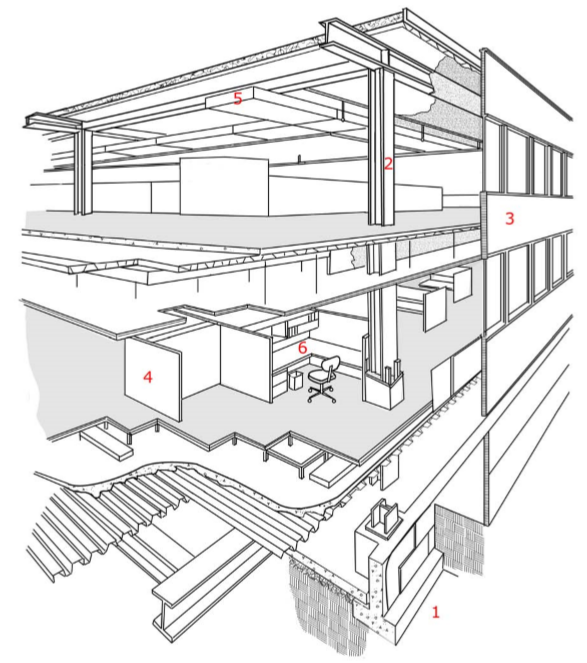
\includegraphics[scale=0.42]{0106}
					\vspace{-.3cm}
					\caption{Curtainwall and raised floor construction. Source: Ruch, Richard, The Building Systems Integration Handbook.}
				\end{figure}
			\end{column}
			\begin{column}{.34\textwidth}
				\begin{enumerate}
					\item Foundation (기초)
					\item Superstructure (상부구조)
					\item Envelope (외피)
					\item Interior partition (내부공간구획)
					\item Mechanical services (설비)
					\item Furnishings (마감)
				\end{enumerate}
			\end{column}
		\end{columns}
	\end{frame}

\section{Architectural Structure}
	\begin{frame}{Architectural Structure}
		\begin{figure}
			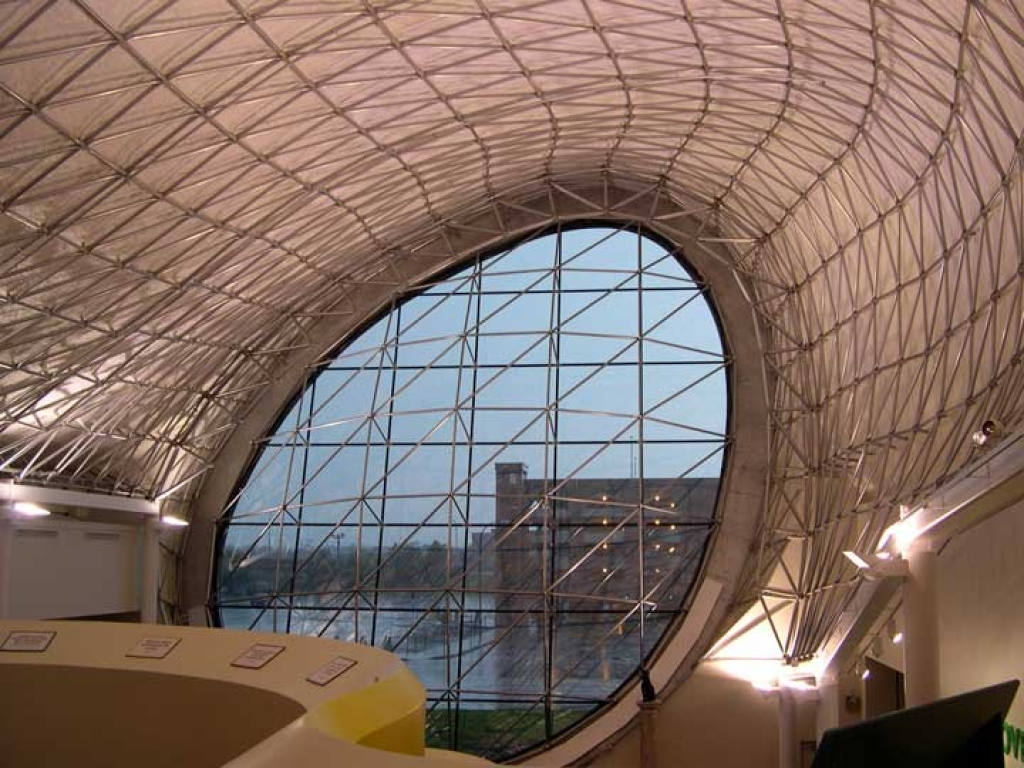
\includegraphics[height=.85\textheight]{01strong}
			\caption{Free Form Roof: Strong Museum, Rochester New York}
		\end{figure}
	\end{frame}
	\begin{frame}{Architectural Structure}
		\begin{figure}
			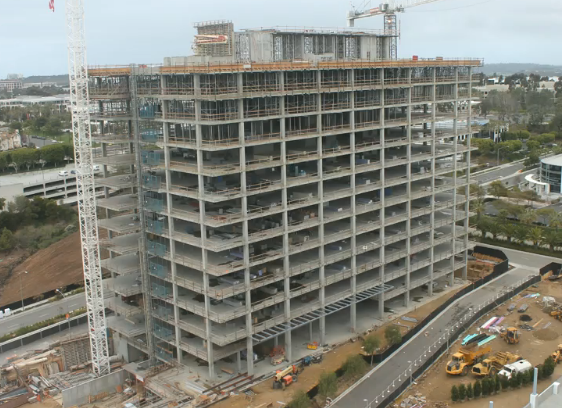
\includegraphics[height=.85\textheight]{01LJC}
			\caption{Typical Building: La Jolla Commons Phase II Office Tower, San Diego}
		\end{figure}		
	\end{frame}
	\begin{frame}{Architectural Structure}
		\textbf{건축구조학의 목적}
		
		\textbf{구조(structure)}: 건축물을 구성하는 요소 가운데 건축물 자체와 적재물의 무게 및 지진이나 풍압력과 같은 건물 외부로부터의 힘에 대한 저항을 주목적으로 설치되는 것. 구체적으로 기둥, 보, 벽 등 건축물의 뼈대.
		
		\textbf{건축구조설계}: 건축물의 기능을 발휘하게 하기 위해 \alert{안정성}, \alert{사용성}, \alert{내구성}을 확보하도록 기획, 설계, 감독하는 작업.
		\vspace{-.3cm}
		\begin{figure}
			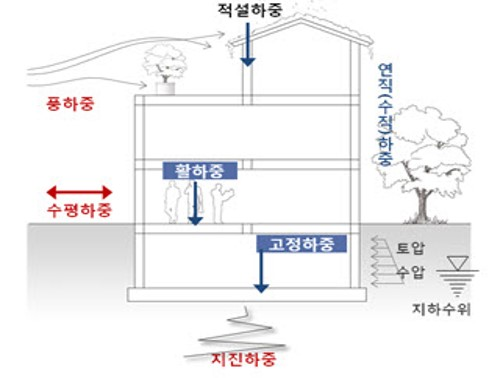
\includegraphics[height=.5\textheight]{01loads}
			\caption{건축물에 작용하는 하중의 종류}
		\end{figure}
	\end{frame}
	\begin{frame}{1.2 건축구조의 분류}
		\textbf{1) 사용재료에 의한 분류}: 구조체에 사용되는 재료는 구성요소로서의 적절한 형상, 치수, 접합법 등을 가지며 그 결과, 구조체 전체로서도 각 재료의 특성이 반영됨. 크게는 목조, \alert{벽돌조}, \alert{철골조}, \alert{철근콘크리트조}, 철골철근콘크리트조, 보강콘크리트블럭조로 구분됨.
		
		\textbf{2) 구성형식에 의한 분류}: 건축구조는 구성방식이나 형상에 따라 \alert{가구식 구조}, \alert{조적식 구조}, \alert{일체식 구조} 등으로 구분됨.
		
		\begin{columns}[t]
			\begin{column}{.33\textwidth}
				\begin{figure}
					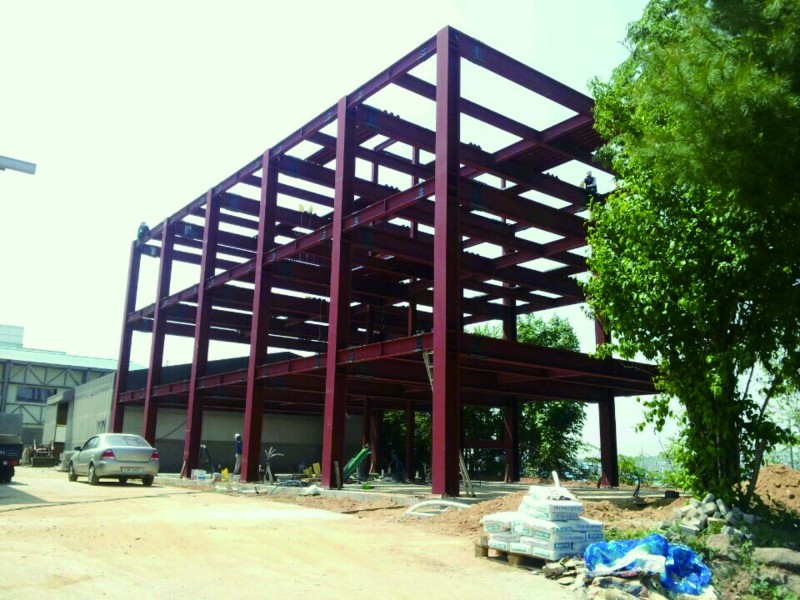
\includegraphics[height=3cm]{01STEEL}
					\caption{철골조건물(가구식)}
				\end{figure}
			\end{column}
			\begin{column}{.33\textwidth}
				\begin{figure}
					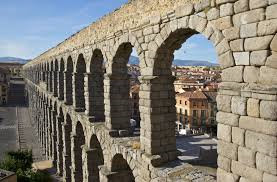
\includegraphics[height=3cm]{01MASONRY}
					\caption{벽돌조건물(조적식)}
				\end{figure}
			\end{column}
			\begin{column}{.33\textwidth}
				\begin{figure}
					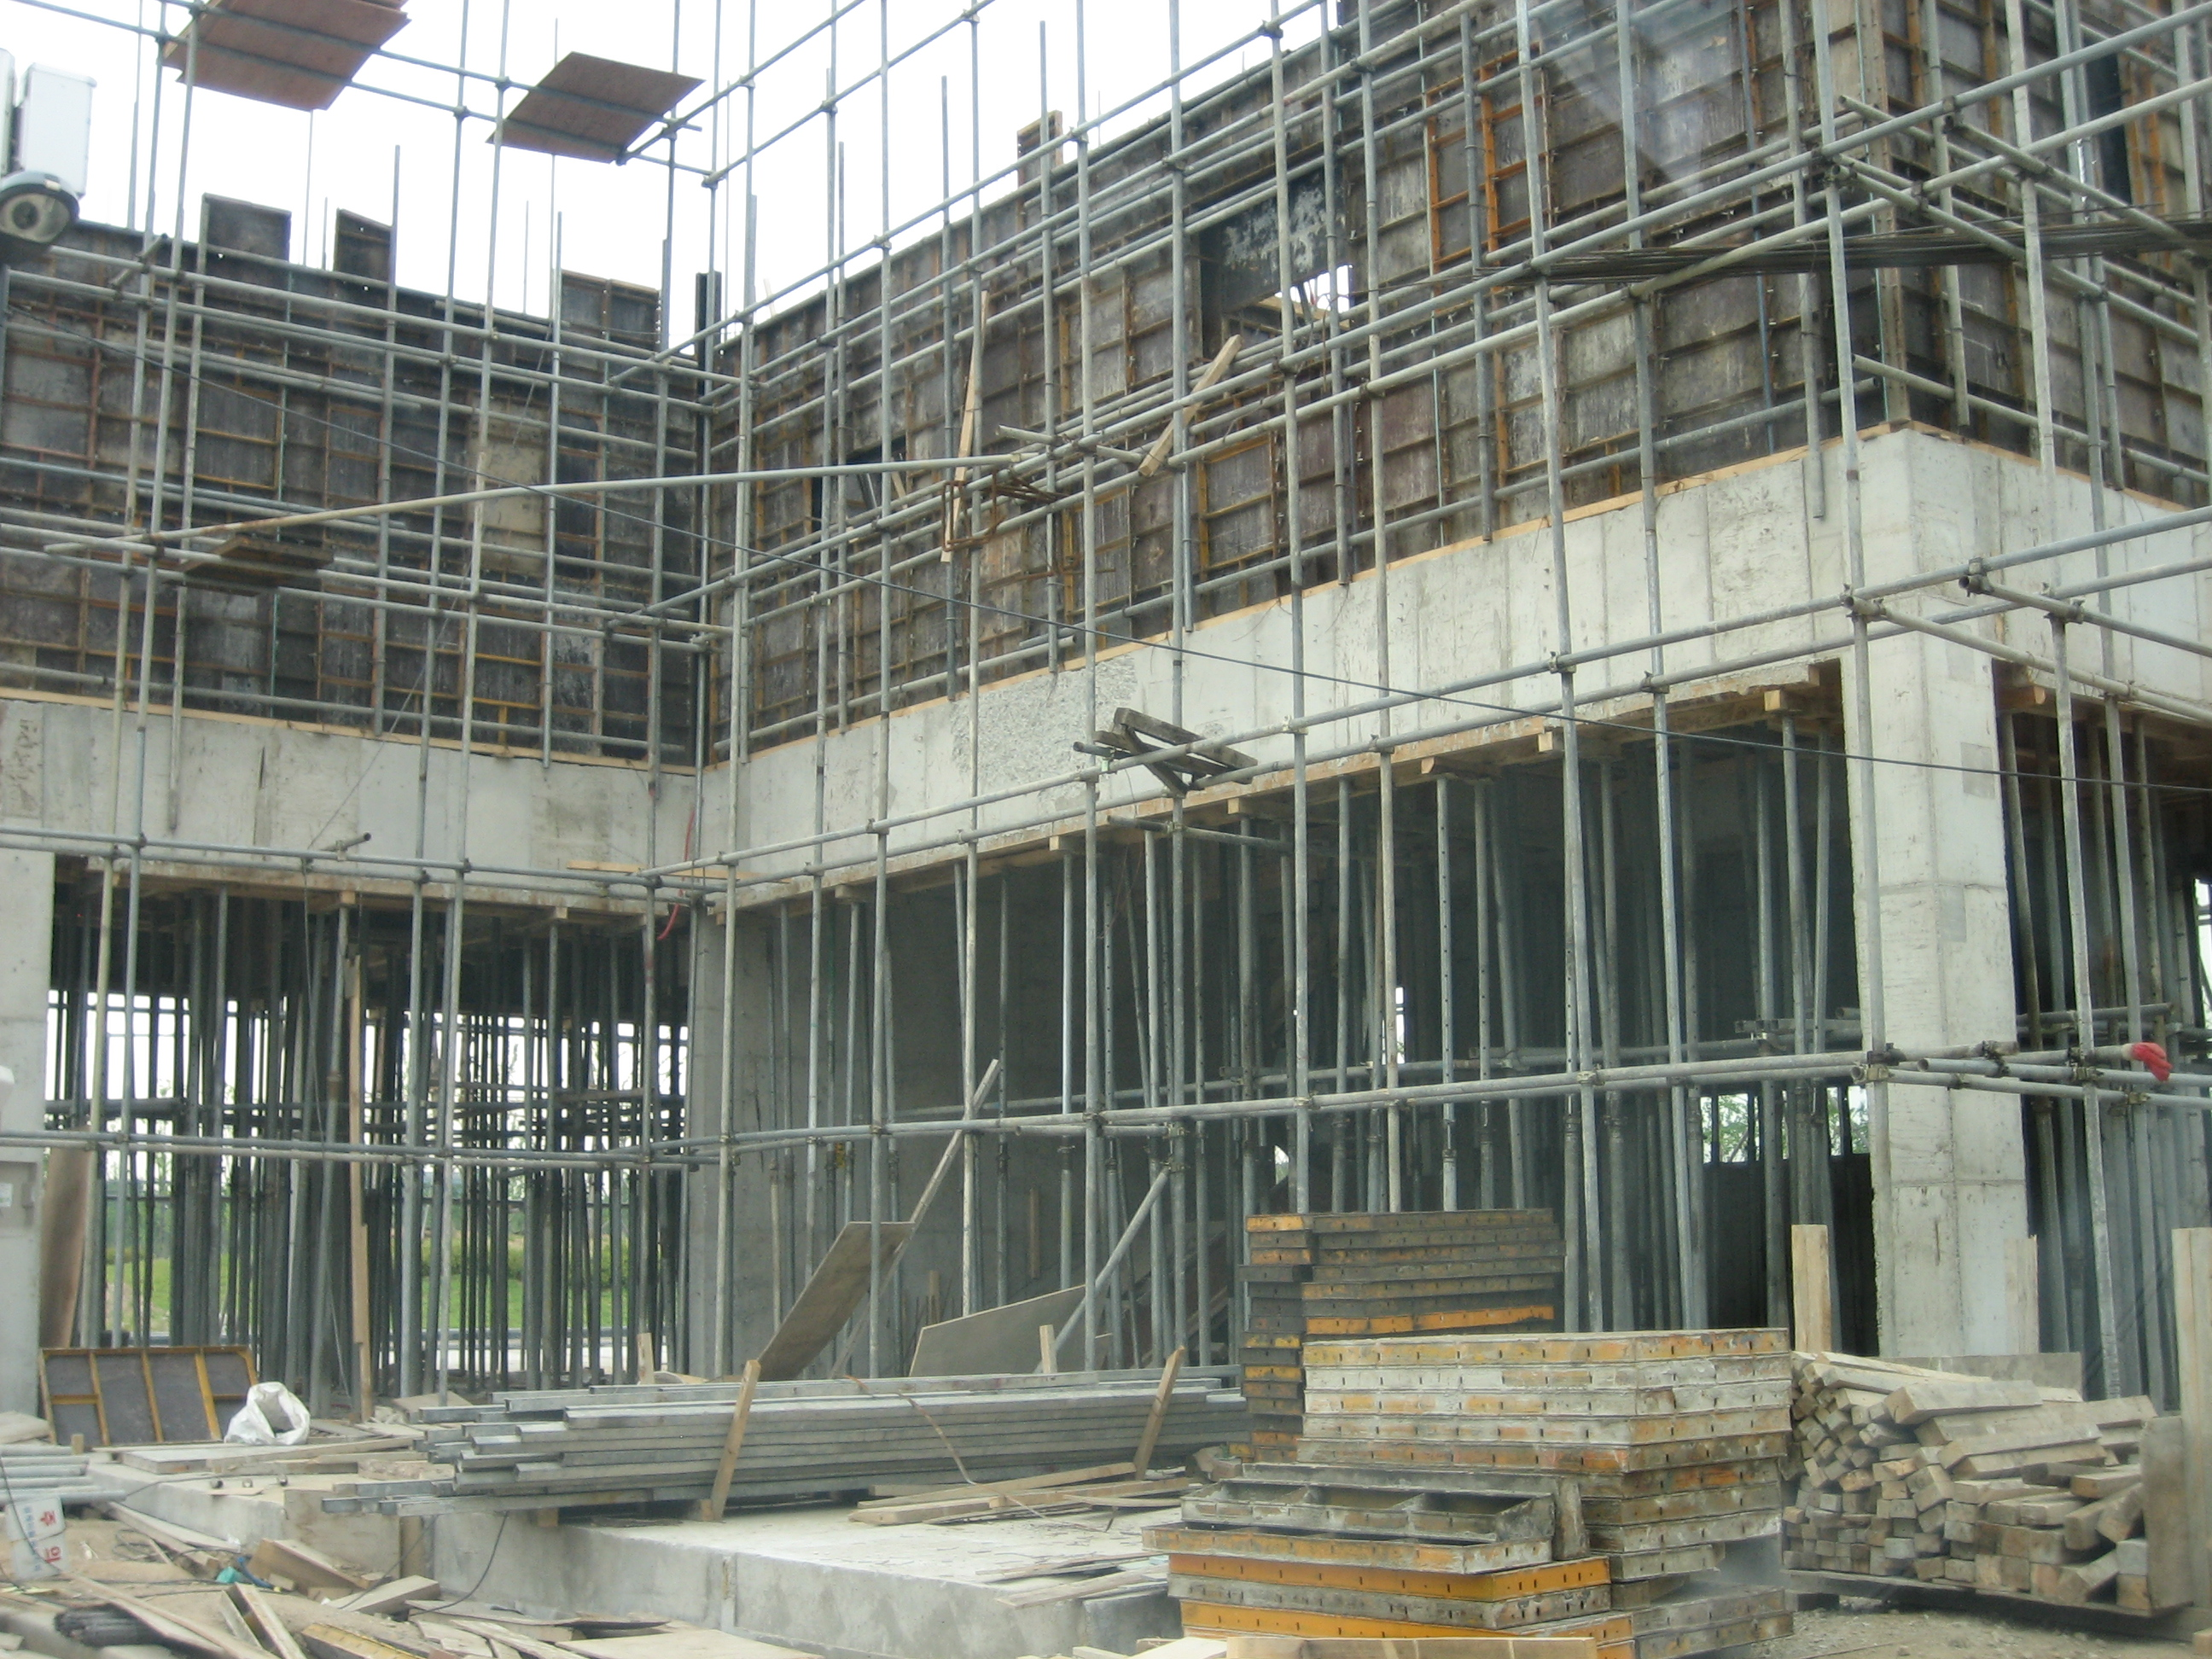
\includegraphics[height=3cm]{01SC}
					\caption{철근콘크리트조건물(일체식)}
				\end{figure}
			\end{column}
		\end{columns}
	\end{frame}
	\begin{frame}{1.3 특수구조}
		대규모 집회장이나 경기장과 같이 \alert{기둥이 없는 넓은 공간}을 만들기 위해 개발된 구조 방법으로 \alert{절판구조}, \alert{쉘구조}, 입체트러스구조, \alert{현수구조}, 막구조 등이 있음. 
		
		\begin{columns}[t]
			\begin{column}{.33\textwidth}
				\begin{figure}
					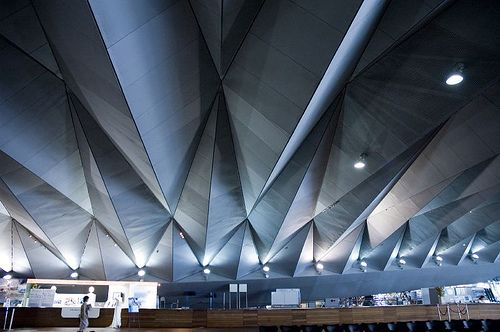
\includegraphics[height=3cm]{01FOLDED}
					\caption{절판구조 일례: Yokohama Port Terminal, Yokohama, Japan}
				\end{figure}
			\end{column}
			\begin{column}{.33\textwidth}
				\begin{figure}
					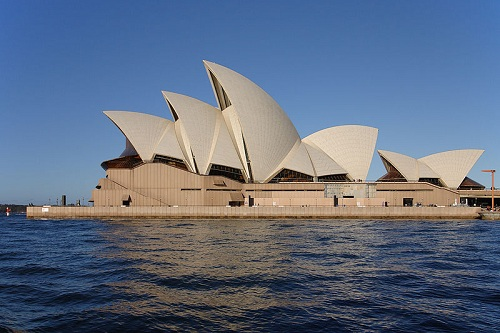
\includegraphics[height=3cm]{01SHELL}
					\caption{쉘구조 일례: Sydney Opera House, Sydney, Austrailia}
				\end{figure}
			\end{column}
			\begin{column}{.33\textwidth}
				\begin{figure}
					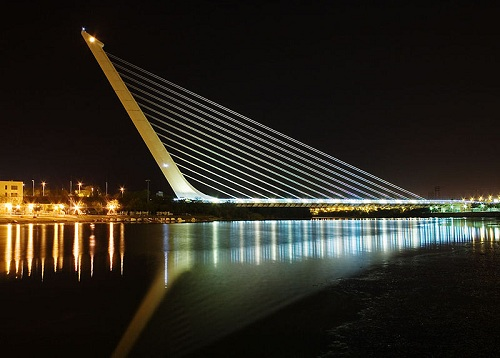
\includegraphics[height=3cm]{01SUSPENDED}
					\caption{현수구조 일례: Alamillo Bridge, Seville, Spain}
				\end{figure}
			\end{column}
		\end{columns}
	\end{frame}
\section{2. 건축구조의 원리}	
	\begin{frame}{2.1 하중과 반력}
		\textbf{2.1.1 하중(load)}: 건축물에 외부로부터 가해지는 힘\alert{(외력, external force)}을 \alert{하중}이라 하며, 이로 인해 건물 내부에 발생하는 힘을 \alert{내력(internal force)}이라 함.
		 
		\textbf{(1) 고정하중(\alert{D})}: \alert{1) 지붕, 기둥, 바닥과 같은 건물의 자중}이나 \alert{2) 고정된 설비 무게} 등. 구성재료의 밀도와 크기, 구성상태에 대한 정보로 \alert{비교적 정확히 파악 가능}. 정하중(dead load)라고도 부름.
		
		\textbf{(2) 적재하중(\alert{L})}: 사람이나 가구, 차량 등의 중량. \alert{재하분포, 크기, 시기가 일정하지 않은 하중}. \alert{고정하중보다 불확실성이 큼}. 동하중(live load)이라고도 부름.
		\begin{exampleblock}{참고: 주요 구조재료의 밀도와 용도별 적재하중}
			\begin{description}
				\item[고정하중] 콘크리트 밀도: 2.4 ton/m$^3$, 강재 밀도: 7.3 ton/m$^3$.
				\item[적재하중] 주거용 건축물의 거실: 2.0 kN/m$^2$, 일반 사무실: 2.5 kN/m$^2$, 문서보관실: 5.0 kN/m$^2$, 도서관 서고: 7.5 kN/m$^2$(건축구조기준, 2016).
			\end{description}
		\end{exampleblock}
	\end{frame}
	\begin{frame}{2.1 하중과 반력}
		\textbf{(3) 적설하중(\alert{S})}: 지붕면에 쌓인 눈의 중량으로 적재하중의 일종. 지역의 적설량과 지붕의 경사도, 난방여부와 관계됨.
		\begin{figure}
			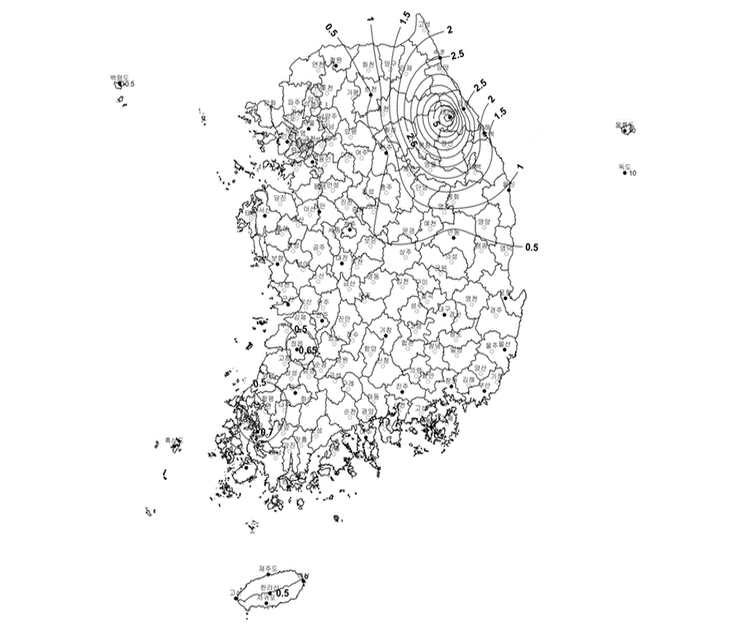
\includegraphics[height=4.5cm]{02SNOW}
			\caption{건축구조기준(2016)에 제시된 기본지상적설하중(kN/m$^2$)}
		\end{figure}
		\vspace{-.5cm}
		\begin{exampleblock}{참고: 지붕의 기울기에 따른 적설하중의 감소계수}
			\vspace{-.3cm}
			\begin{table}[]
				\centering
				\begin{tabular}{@{}ccccc@{}}
				\toprule
				 지붕의 경사 & 10\textdegree$\sim$20\textdegree & 20\textdegree$\sim$30\textdegree & 30\textdegree$\sim$40\textdegree & 40\textdegree$\sim$60\textdegree \\
				 \midrule
				 감소계수 & 0.90 & 0.75 & 0.50 & 0.25 \\
				 \bottomrule
				\end{tabular}
			\end{table}
		\end{exampleblock}
	\end{frame}
	\begin{frame}{2.1 하중과 반력}
		\textbf{(4) 풍하중(\alert{W})}: 건물의 외벽 또는 지붕에 미치는 바람의 압력.

		\vspace{-.3cm}
		\begin{columns}[t]
			\begin{column}{.6\textwidth}
				\begin{figure}
					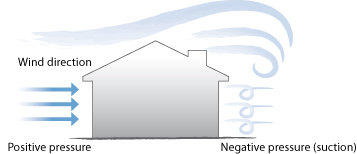
\includegraphics[scale=0.5]{01Windload}
					\caption{풍하중의 전형적 패턴 일례}
				\end{figure}
			\end{column}
			\begin{column}{.39\textwidth}
				\begin{figure}
					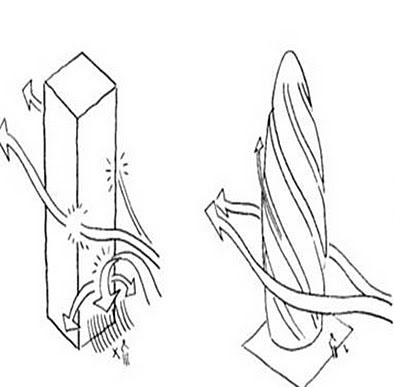
\includegraphics[scale=0.3]{01AD}
					\caption{풍동역학적 특성을 고려해 디자인된 건물의 풍하중 경감}
				\end{figure}
			\end{column}
		\end{columns}
	\end{frame}
	\begin{frame}{2.1 하중과 반력}
		\textbf{(5) 지진하중(\alert{K})}: 건물의 기초나 상부구조물에 미치는 지진의 힘. 국내의 경우 강진의 발생확률은 희박하지만 파국적 피해를 고려할 때 내진설계가 반드시 필요. 
		\vspace{-.5cm}
		\begin{columns}[t]
			\begin{column}{.6\textwidth}
				\begin{figure}
					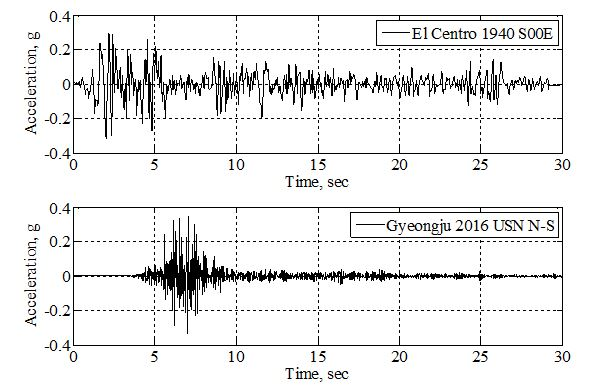
\includegraphics[scale=0.4]{01EH}
					\caption{지진기록 비교: El Centro (1940) vs. Gyeong-Ju (2016)}
				\end{figure}
			\end{column}
			\begin{column}{.39\textwidth}
				\begin{figure}
					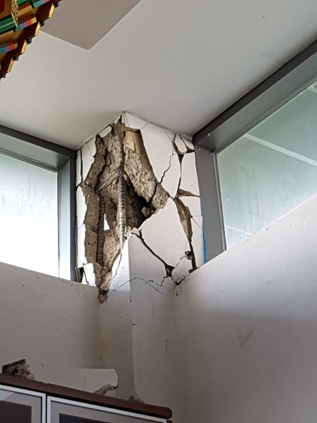
\includegraphics[scale=0.7]{01KJ}
					\caption{경주지진에 의한 피해 사례}
				\end{figure}
			\end{column}
		\end{columns}
	\end{frame}
	\begin{frame}{구조물의 붕괴사례}
		\textbf{삼풍백화점 붕괴사고}: 1995년 6월 29일 오후 5시 57분에 발생한 한국 역사상 최악의 건축물 붕괴사고. 
		\vspace{-.7cm}
		\begin{columns}[t]
			\begin{column}{.6\textwidth}
				\begin{figure}
					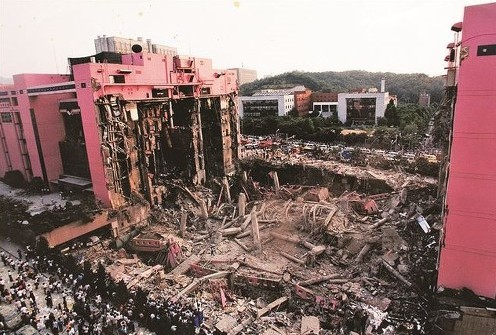
\includegraphics[scale=0.55]{01SPT}
					\caption{삼풍백화점 붕괴사고}
				\end{figure}
			\end{column}
			\begin{column}{.49\textwidth}
				\begin{figure}
					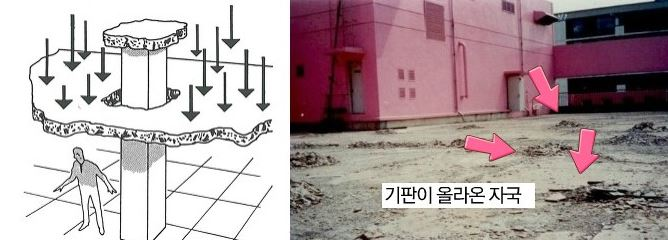
\includegraphics[scale=0.3]{01SP}		
				\end{figure}
			\end{column}
		\end{columns}
	\end{frame}
	\begin{frame}{구조물의 붕괴사례}
		\textbf{경주 마우나리조트 붕괴사고}: 2014년 2월 17일 오후 9시 11분 무렵, 경주시 양남면 신대리 마우나오션리조트의 강당 건물이 폭설로 무너져 내려 새내기 오리엔테이션을 진행 중이던 부산외국어대학교 학생들이 매몰돼 10명의 사망자와 204명의 부상자를 발생시킨 대형 참사. 
		\begin{columns}[t]
			\begin{column}{.55\textwidth}
				\begin{figure}
					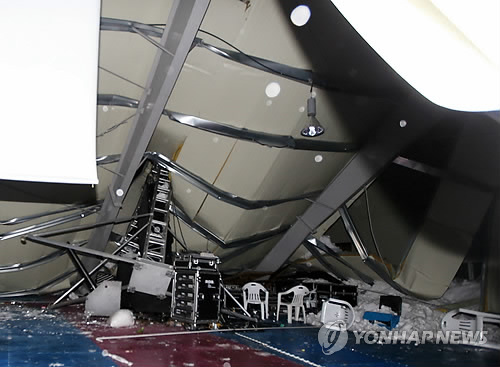
\includegraphics[scale=0.3]{01MR}
					\caption{마우나리조트 천장 붕괴현장}
				\end{figure}
			\end{column}
			\begin{column}{.44\textwidth}
				\begin{figure}
					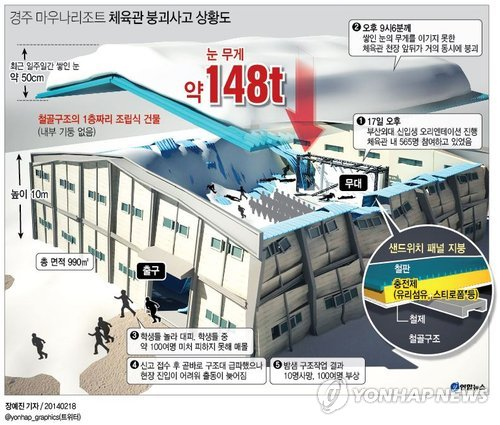
\includegraphics[scale=0.4]{01MR2}
					\caption{붕괴사고 상황도}
				\end{figure}
			\end{column}
		\end{columns}
	\end{frame}
\end{document}
